\begin{figure}[ht]
\tikzset{black/.style={shape=circle,draw=black,fill=black,inner sep=1pt, minimum size=9pt}}
\tikzset{white/.style={shape=circle,draw=black,fill=white,inner sep=1pt, minimum size=9pt}}

\tikzset{invisible/.style={shape=circle,draw=black,fill=black,inner sep=0pt, minimum size=0.1pt}}
\begin{center}
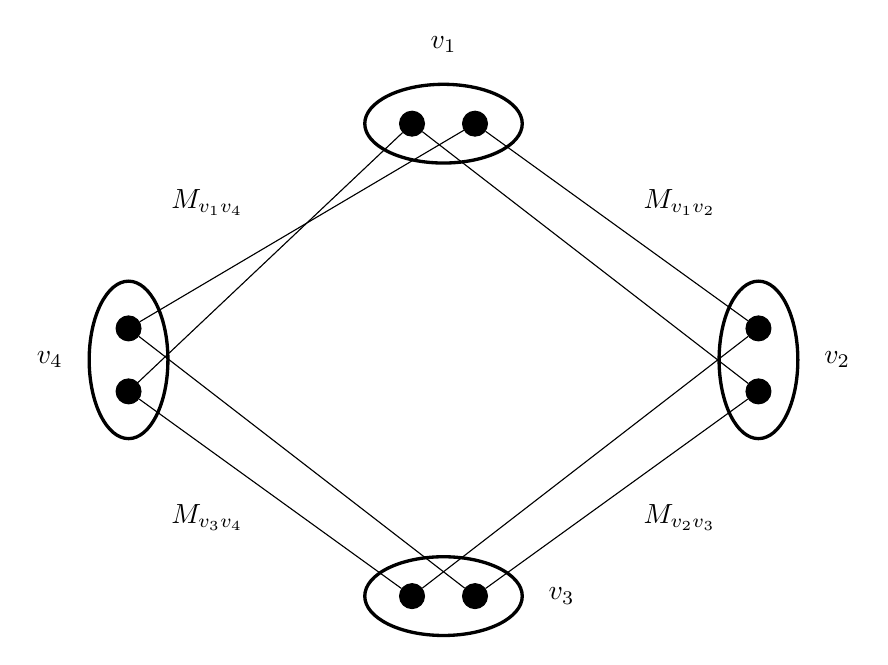
\begin{tikzpicture}
\filldraw[color=black!100, fill=black!0, very thick] (0,-3) ellipse (1 and 0.5);
\filldraw[color=black!100, fill=black!0, very thick] (4,0) ellipse (0.5 and 1);
\filldraw[color=black!100, fill=black!0, very thick] (-4,0) ellipse (0.5 and 1);
\filldraw[color=black!100, fill=black!0, very thick] (0,3) ellipse (1 and 0.5);
        \node[] at (-5,0) {$v_4$};
        \node[] at (1.5,-3) {$v_3$};
        \node[] at (5,0) {$v_2$};
        \node[] at (0,4) {$v_1$};
        
        \node[] at (-3,2) {$M_{v_1v_4}$};
        \node[] at (3,-2) {$M_{v_2v_3}$};
        \node[] at (3,2) {$M_{v_1v_2}$};
        \node[] at (-3,-2) {$M_{v_3v_4}$};

        \node[black] (1) at (-0.4,3){};
        \node[black] (2) at (0.4,3){};
        
        \node[black] (3) at (4,0.4){};
        \node[black] (4) at (4,-0.4){};

        \node[black] (5) at (0.4,-3){};
        \node[black] (6) at (-0.4,-3){};

        \node[black] (7) at (-4,-0.4){};
        \node[black] (8) at (-4,0.4){};

      

        \draw[black] (1)--(4); 
        \draw[black] (2)--(3); 
        \draw[black] (3)--(6); 
        \draw[black] (4)--(5); 
        \draw[black] (5)--(8); 
        \draw[black] (6)--(7); 
        \draw[black] (1)--(7); 
        \draw[black] (2)--(8); 
 

\end{tikzpicture}


\caption{An illustration of a 4-cycle $v_1v_2v_3v_4v_1$ together with a 2-correspondence $(L,M)$ for which the 4-cycle does not admit an $(L,M)$-colouring. Each oval represents a vertex in the 4-cycle. The dots within these vertices represent the colours in vertices' lists. The edges between vertices correspond to the matchings in $M$.} 
    \label{fig:c4ex}
\end{center}
\end{figure}






